\section{Sơ đồ ERD mức khái niệm}

\begin{figure}[H]
    \centering
    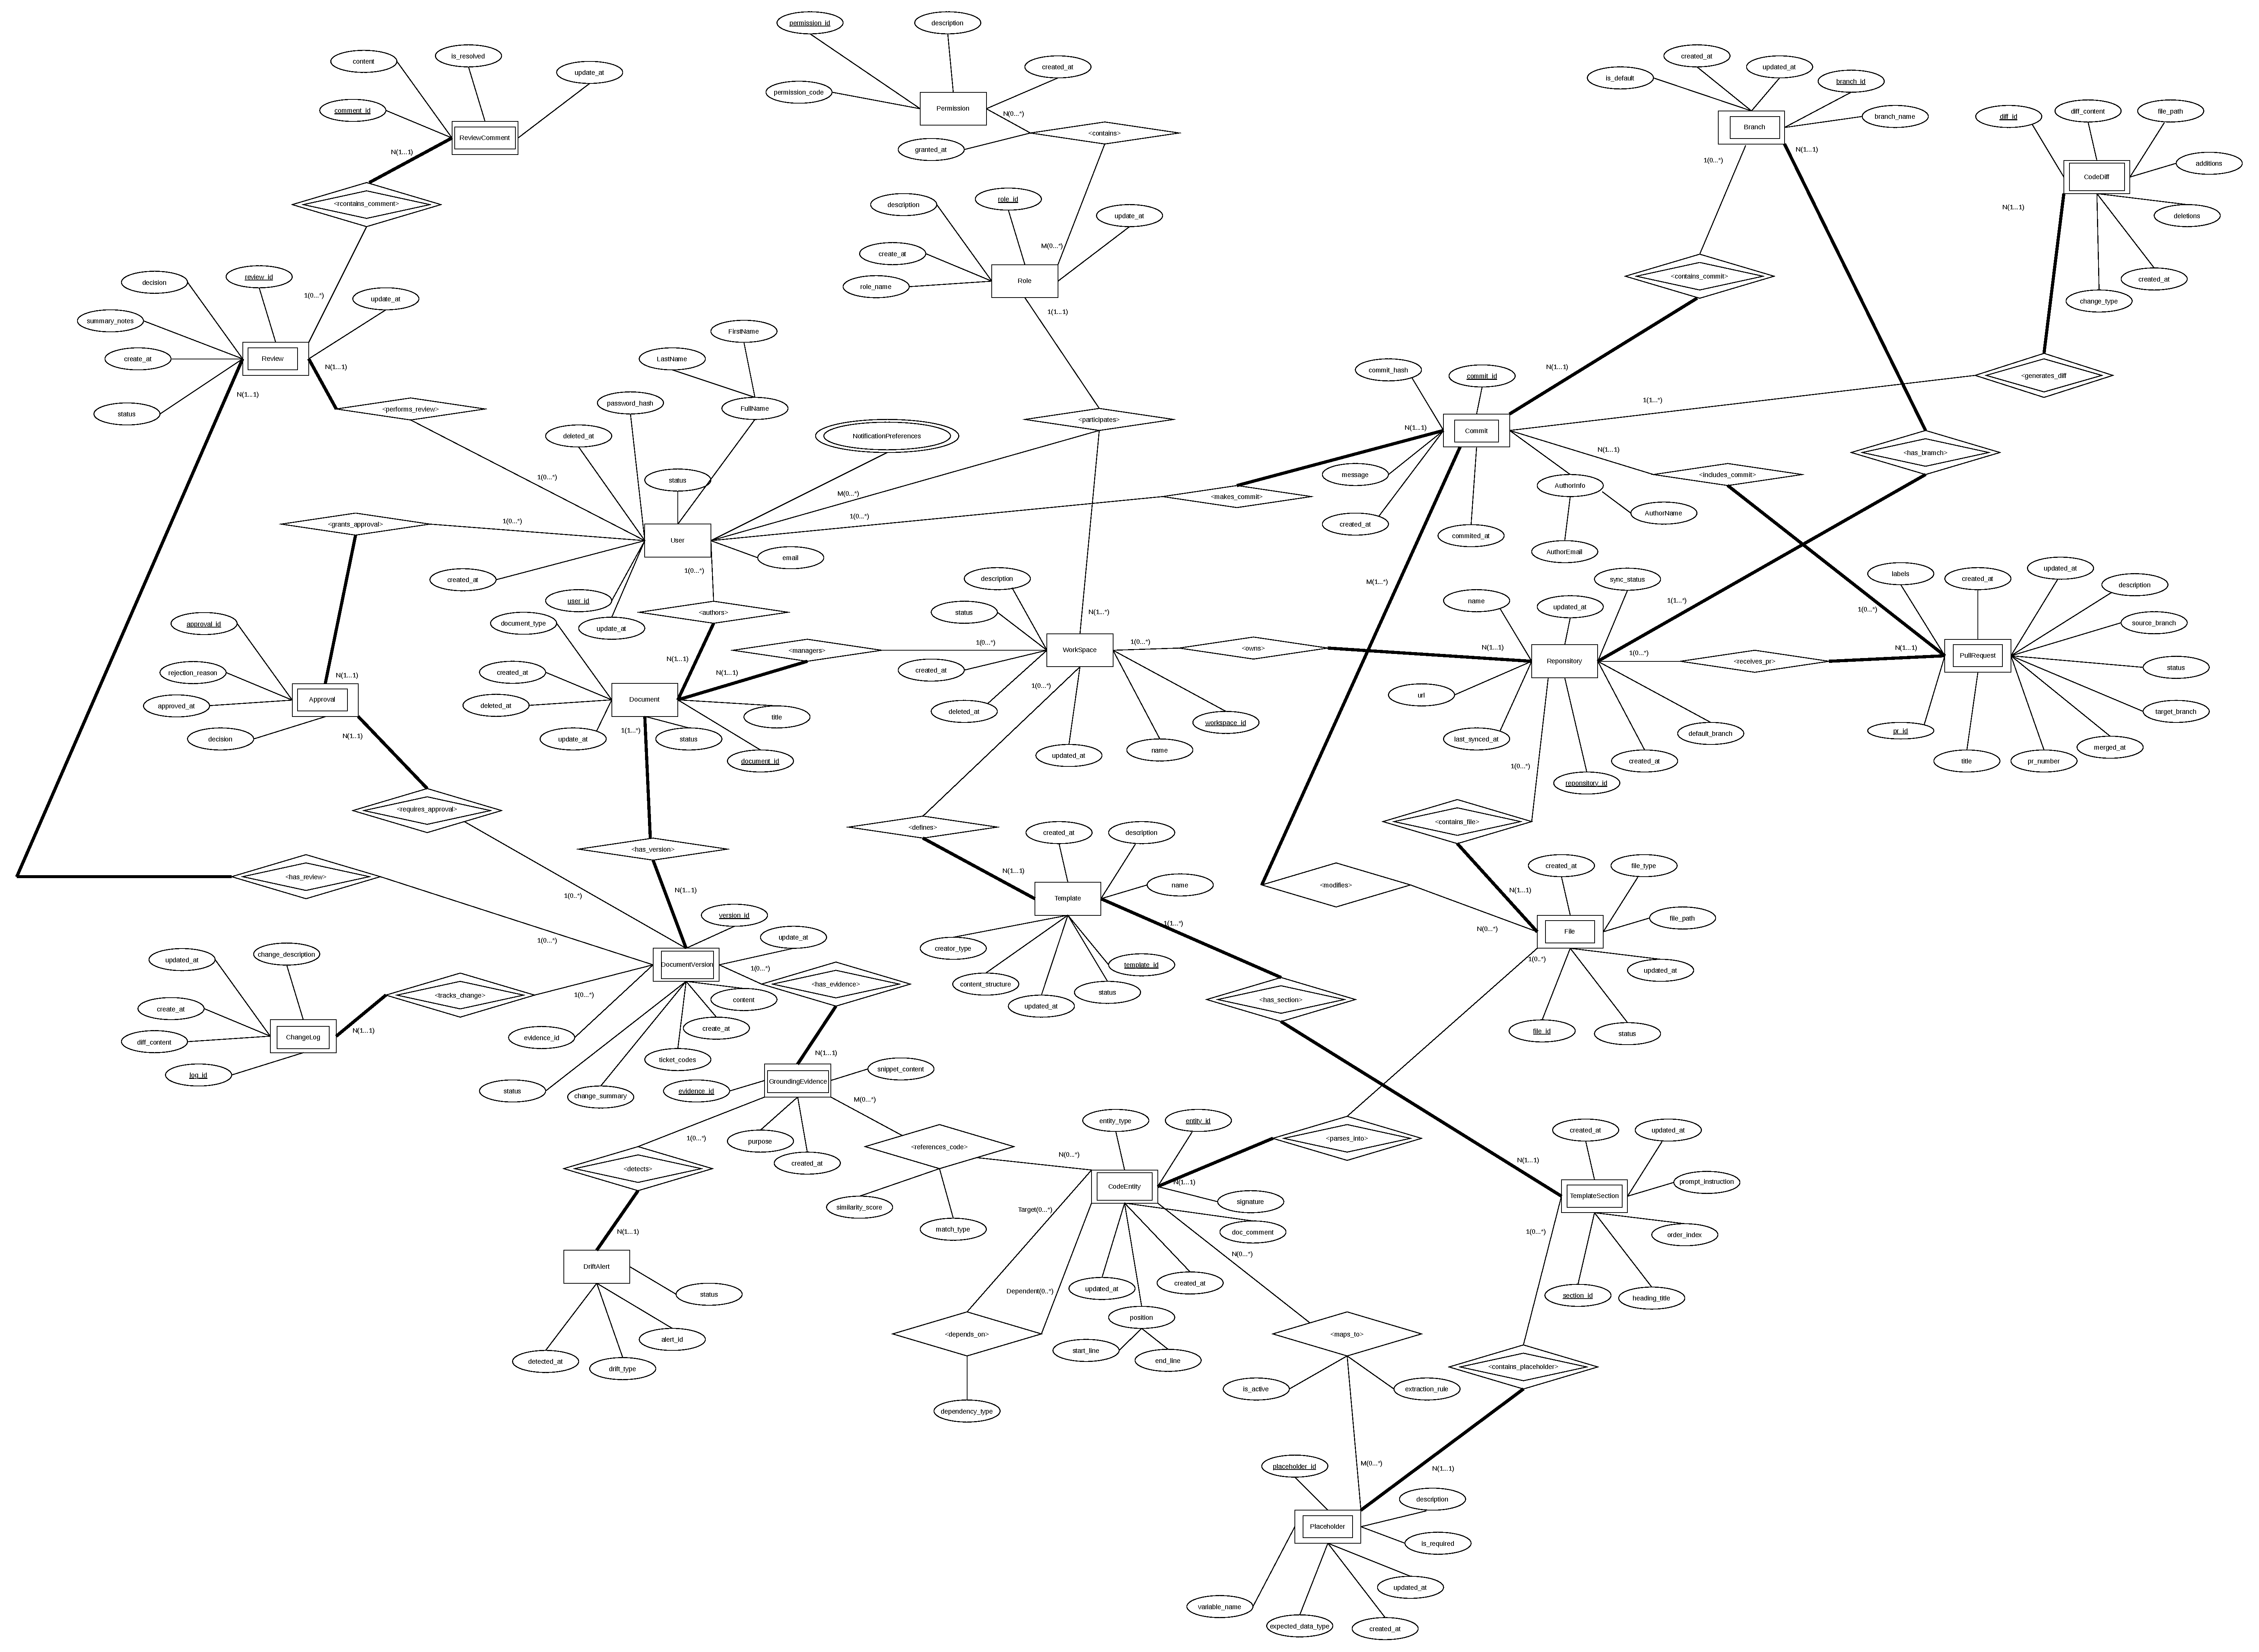
\includegraphics[
        width=\textwidth,
        height=0.75\textheight,
        keepaspectratio
    ]{./images/erd_muckhainiem.pdf}
    \caption{Sơ đồ ERD mức khái niệm}
    \label{fig:erd-conceptual}
\end{figure}
\noindent
Sơ đồ ERD mức khái niệm đã phác họa một cách toàn diện và chặt chẽ kiến trúc dữ liệu tổng quan cho Hệ thống Quản lý và Đồng bộ Tài liệu Kỹ thuật với Mã nguồn Dự án Phần mềm. Sơ đồ này không chỉ là bản thiết kế tĩnh về lưu trữ, mà còn phản ánh luồng nghiệp vụ khép kín, giải quyết bài toán cốt lõi: duy trì sự thống nhất và minh bạch giữa tài liệu kỹ thuật và mã nguồn thực tế trong suốt vòng đời phát triển phần mềm (SDLC).
Mô hình dữ liệu được phân rã một cách có hệ thống thành bốn nhóm phân hệ nghiệp vụ trọng tâm, có tính liên kết chặt chẽ với nhau:
Phân hệ Quản trị Người dùng, Định danh và Tổ chức Không gian làm việc: Hệ thống bắt đầu bằng việc thiết lập nền tảng bảo mật và tổ chức công việc đa người dùng. Cấu trúc dữ liệu cho phép xác thực người dùng chặt chẽ, gán vai trò và phân quyền truy cập chi tiết. Sau khi đăng nhập, người dùng sẽ khởi tạo và quản lý các Workspace (Không gian làm việc). Đây là các ranh giới luận lý giúp tổ chức dự án, cô lập tài nguyên và làm tiền đề cho việc tích hợp với các kho lưu trữ bên ngoài.
Phân hệ Tích hợp, Trích xuất và Quản lý Tri thức Mã nguồn: Từ không gian làm việc, các Repository (Kho chứa mã) được kết nối trực tiếp với hệ sinh thái quản lý phiên bản thông qua GitHubConnection. Luồng dữ liệu tự động đồng bộ liên tục các siêu dữ liệu quan trọng bao gồm: Branch (Nhánh phát triển), Commit (Lịch sử thay đổi), PullRequest (Yêu cầu gộp mã) và CodeDiff (Chi tiết các dòng mã thay đổi). Từ các File bị tác động, hệ thống thực hiện phân tích cú pháp để bóc tách thành các CodeEntity (Thực thể mã nguồn như hàm, lớp, biến). Các CodeEntity này đóng vai trò là lõi tri thức của hệ thống, biến mã nguồn thô thành dữ liệu có cấu trúc để sẵn sàng phục vụ cho việc sinh tài liệu.
Phân hệ Tự động Sinh tài liệu và Truy vết Bằng chứng (Traceability): Đây là trái tim của hệ thống, nơi tài liệu kỹ thuật được xây dựng không phải bằng phương pháp thủ công mà thông qua cơ chế tự động hóa dựa trên ngữ cảnh (context-aware). Hệ thống cung cấp các Template (Khuôn mẫu) được thiết kế theo các tiêu chuẩn ngành, bao gồm nhiều TemplateSection (Phân hệ nội dung) và các Placeholder (Biến định vị). Thay vì điền tay, dữ liệu từ các CodeEntity sẽ được ánh xạ động vào các Placeholder này để sinh ra các Document (Tài liệu) hoàn chỉnh. Đặc biệt, sự liên kết này được hiện thực hóa thông qua các GroundingEvidence (Bằng chứng truy vết), giúp người đọc luôn biết chính xác đoạn văn bản nào đang mô tả cho đoạn code (hoặc kiến trúc) nào, đảm bảo nội dung tài liệu luôn có cơ sở thực tế và tính chính xác tuyệt đối.
Phân hệ Kiểm soát Sai lệch (Drift Detection), Quản lý Phiên bản và Kiểm duyệt: Để giải quyết triệt để tình trạng "tài liệu bị lỗi thời", sơ đồ ERD đã định nghĩa một cơ chế giám sát vòng đời tài liệu nghiêm ngặt. Mỗi khi kho mã nguồn có biến động (commit mới), hệ thống sẽ đối chiếu và tự động phát sinh các DriftAlert (Cảnh báo sai lệch) nếu phát hiện tài liệu hiện hành không còn phản ánh đúng thực trạng mã nguồn. Mọi thay đổi trong nội dung tài liệu đều được theo dõi chặt chẽ thông qua DocumentVersion (Phiên bản tài liệu) và lưu vết tại ChangeLog (Lịch sử thay đổi). Cuối cùng, trước khi một phiên bản tài liệu được hợp thức hóa và ban hành, nó buộc phải đi qua một quy trình kiểm duyệt nhiều bước bao gồm Review (Đợt đánh giá), ReviewComment (Góp ý chi tiết) và Approval (Phê duyệt).
Nhìn một cách tổng thể, sơ đồ ERD mức khái niệm này đã tái hiện thành công một luồng dữ liệu khép kín: từ khâu tổ chức và cấp phép truy cập, đồng bộ và phân tích mã nguồn sâu, cho đến quy trình sinh tài liệu tự động hóa và giám sát vòng đời chặt chẽ. Cấu trúc dữ liệu này vượt xa yêu cầu lưu trữ thông tin đơn thuần; nó thiết lập một bộ quy tắc logic vững chắc giúp hiện thực hóa tầm nhìn của dự án là loại bỏ khoảng cách giữa code và document, đảm bảo tính đồng bộ, minh bạch và tin cậy cao nhất cho mọi dự án phần mềm.



\section{Sơ đồ Class}

\begin{figure}[H]
    \centering
    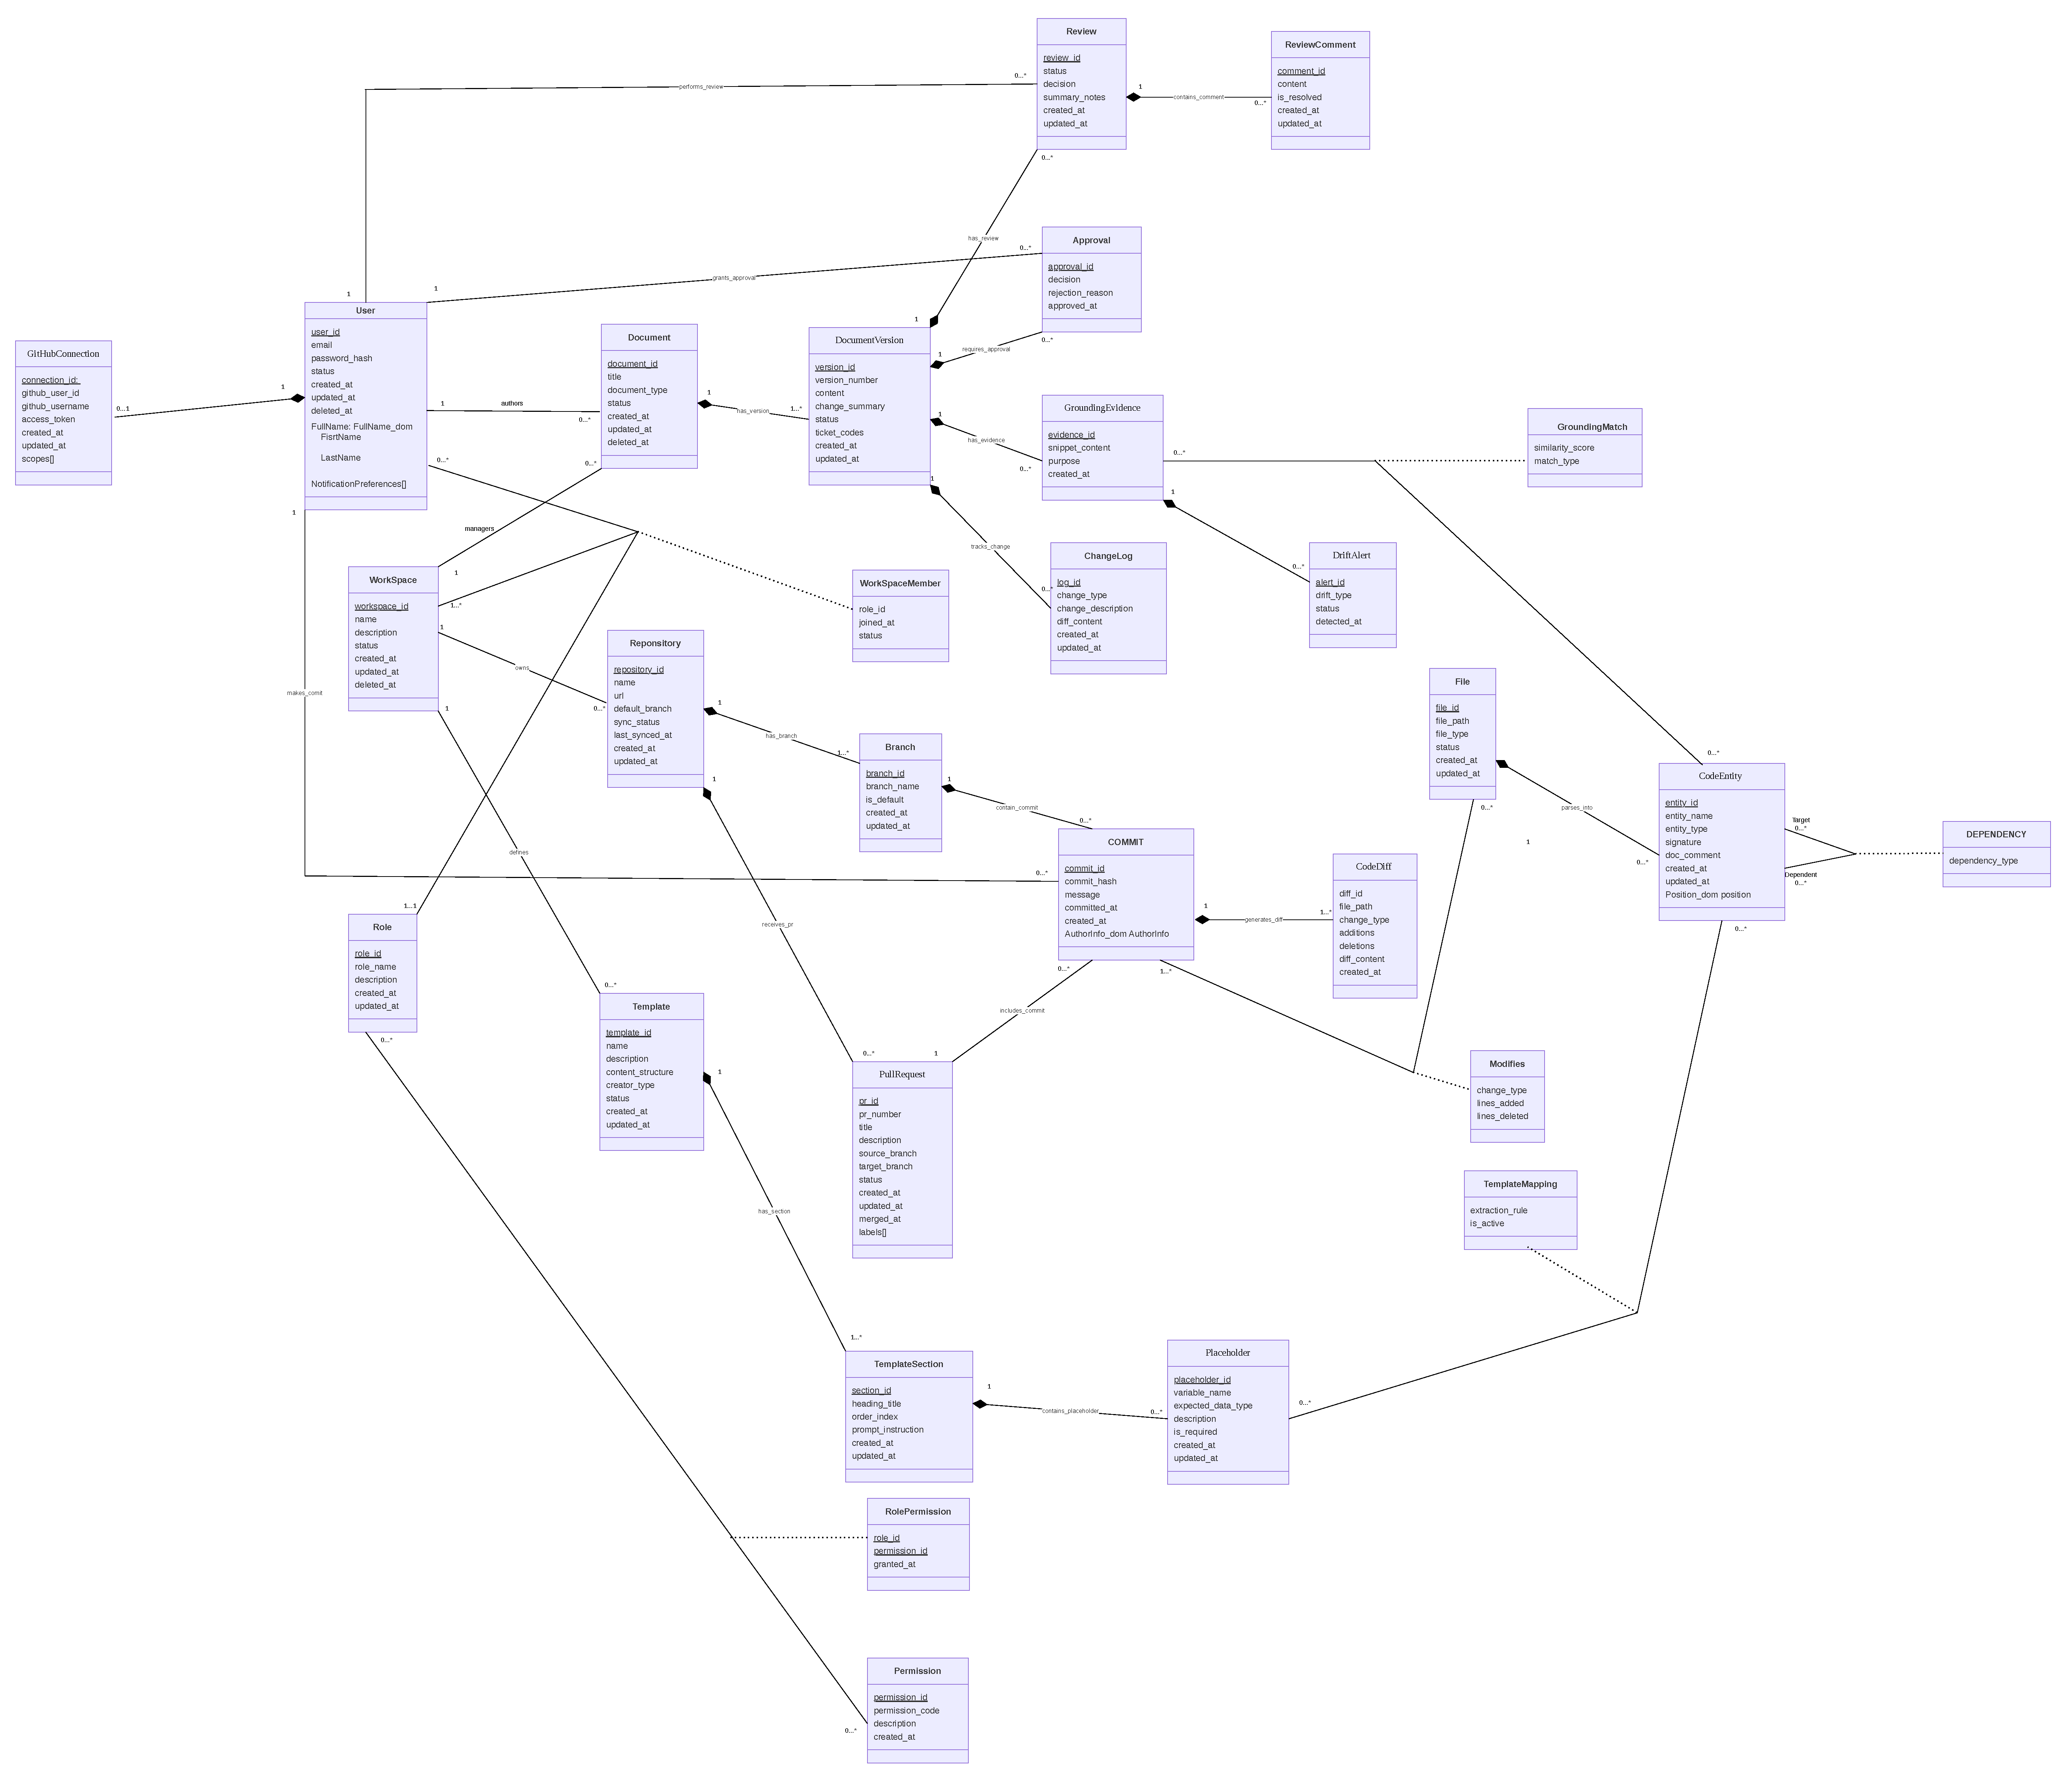
\includegraphics[
        width=\textwidth,
        height=0.75\textheight,
        keepaspectratio
    ]{./images/class.pdf}
    \caption{Sơ đồ Class}
    \label{fig:class-diagram}
\end{figure}
\noindent
Sơ đồ Lớp (Class Diagram) phác họa chi tiết cấu trúc tĩnh của tầng miền nghiệp vụ (Domain Layer) thuộc Hệ thống Quản lý và Đồng bộ Tài liệu Kỹ thuật với Mã nguồn, được phân hoạch rõ ràng thành sáu nhóm chức năng chuyên biệt. Nhóm quản trị định danh và tổ chức xoay quanh các lớp User, Role, Permission và WorkSpace, chịu trách nhiệm thiết lập bảo mật và không gian làm việc luận lý. Nhóm tích hợp mã nguồn gồm GitHubConnection, Repository, Branch, Commit, PullRequest, CodeDiff, File và CodeEntity, giúp mô hình hóa việc kết nối và đồng bộ dữ liệu từ hệ thống quản lý phiên bản. Việc định nghĩa cấu trúc tài liệu được đảm nhận bởi nhóm khuôn mẫu (Template, TemplateSection, Placeholder), trong khi nội dung thực tế và lịch sử biến động được kiểm soát chặt chẽ bởi nhóm quản lý vòng đời tài liệu (Document, DocumentVersion, ChangeLog). Quá trình kiểm soát chất lượng trước khi ban hành được chuẩn hóa qua nhóm quy trình đánh giá (Review, ReviewComment, Approval), và cuối cùng là nhóm giám sát đồng bộ (DriftAlert) giúp cảnh báo mọi sai lệch giữa tài liệu và thực trạng mã nguồn. 
Về mặt nguyên lý thiết kế hướng đối tượng, hệ thống thể hiện rõ tính đóng gói (Encapsulation) và trách nhiệm đơn lẻ (Single Responsibility), trong đó mỗi lớp chỉ nắm giữ tập thuộc tính và trạng thái thuộc phạm vi trách nhiệm của riêng mình. Thay vì để các thuộc tính rời rạc trên lớp chủ, thiết kế ưu tiên sử dụng các Đối tượng Giá trị (Value Object) như FullName\_dom, AuthorInfo\_dom hay Position\_dom để đóng gói các nhóm thuộc tính có liên quan chặt chẽ về mặt ngữ nghĩa (như họ tên, thông tin tác giả, tọa độ mã nguồn), giúp làm sạch lớp thực thể chính và tăng tính tái sử dụng. Đặc biệt, các mối quan hệ nhiều - nhiều mang thuộc tính riêng đã được mô hình hóa thành các Lớp liên kết (Association Class) độc lập như RolePermission, WorkSpaceMember, GroundingMatch, TemplateMapping, Modifies và Dependency. Kỹ thuật quan trọng này giúp tách bạch hoàn toàn bản thể dữ liệu cốt lõi khỏi siêu dữ liệu mô tả mối quan hệ, qua đó giải quyết bài toán mở rộng ngữ nghĩa (ví dụ: một biến giữ chỗ khớp với thực thể mã với độ tương đồng bao nhiêu) một cách an toàn mà không làm phình to hay rối rắm cấu trúc của các lớp gốc. 

